\documentclass[times, utf8, seminar]{fit}

\usepackage{listings}
\usepackage{longtable}
\usepackage{xcolor}
\usepackage{float}
\usepackage{enumitem}
\usepackage{hyperref}
\usepackage{enumerate}
\usepackage{graphicx}
\usepackage{etoolbox}
\usepackage{datetime}
\usepackage{needspace}
\usepackage{titlesec}

\begin{document}
\widowpenalty=300
\clubpenalty=300
\setlength{\parindent}{0pt}

\lstset{
  language=bash,
  backgroundcolor=\color{gray!25},
  basicstyle=\ttfamily \footnotesize,
  breaklines=true,
  prebreak=\raisebox{0ex}[0ex][0ex] {\ensuremath{\hookleftarrow}},
  columns=fullflexible,
  keywords={},
  mathescape=false
}

\title{Agilni \emph{software development}\newline \emph{toolbox}}

\author{Ernad Husremović}
\brindex{DL 2792}
\verzija {0.3.0}
\mentor{mr. Adil Joldić}

\maketitle

\tableofcontents

%\listoftables
%\listoffigures
\newpage

% abstract begin
%\begin{abstract}
%
%To be done 
%
%\keywords{open source software, OSS, Bosna i Hercegovina}
%\end{abstract}

% abstract end

\chapter{Uvod}

Materijal sadrži \emph{Case-study}  alata i servisa koje koristi firma ''bring.out'' doo Sarajevo za potrebe razvoja software-a.

\chapter{Upravljanje i praćenje projekata i tekućih operacija}

\section{Trello projekt menadžment}

\begin{itemize}
      \item \href{https://trello.com/board/f18-knowhow-erp/50af43adf5c6f78820000223}{\color{blue}{F18 trello}}
      \item \href{https://trello.com/board/agilni-toolset-infrastruktura/50af48a4c8ddb2bf32012f47}{\color{blue}{Agilni toolset}}
      \item \href{https://trello.com/board/r-d/50af8dd450a1b0e36a0056fb}{\color{blue}{Research \& development (R\&D)}}
\end{itemize}

\begin{figure}[H]
\centering
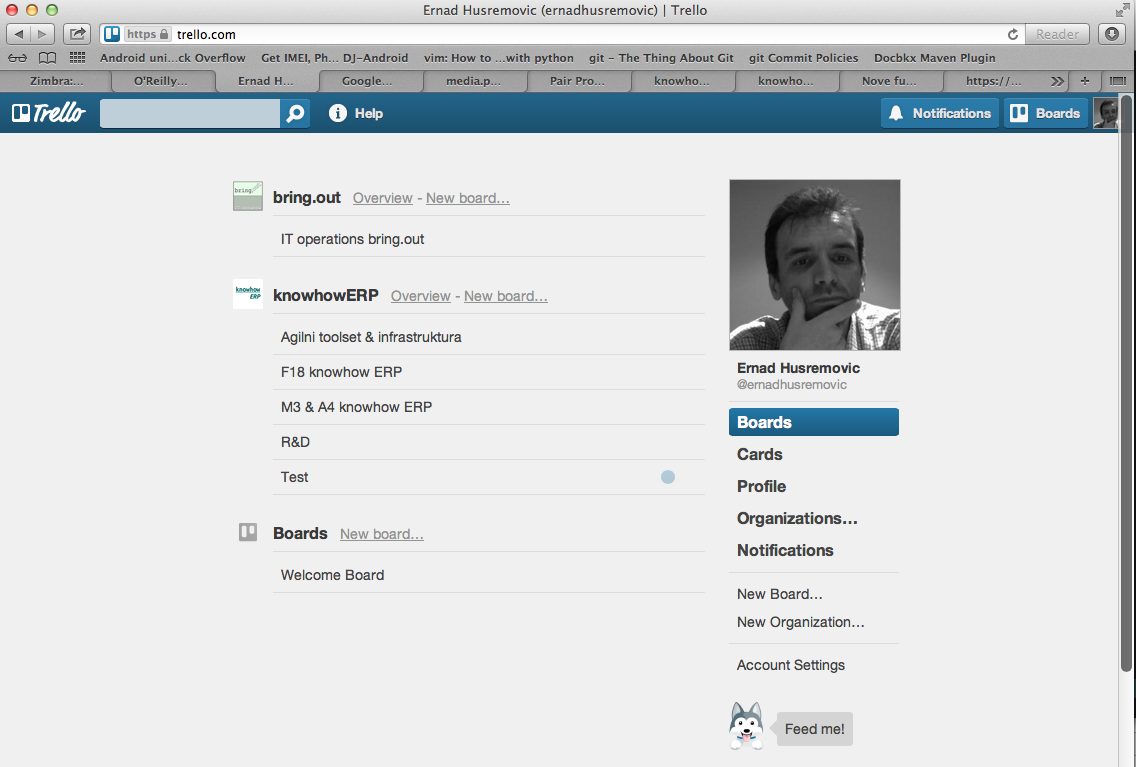
\includegraphics[width=14cm]{img/trello_dashboard.png}
\caption{Trello ''dashboard''}
\end{figure}


\begin{figure}[H]
\centering
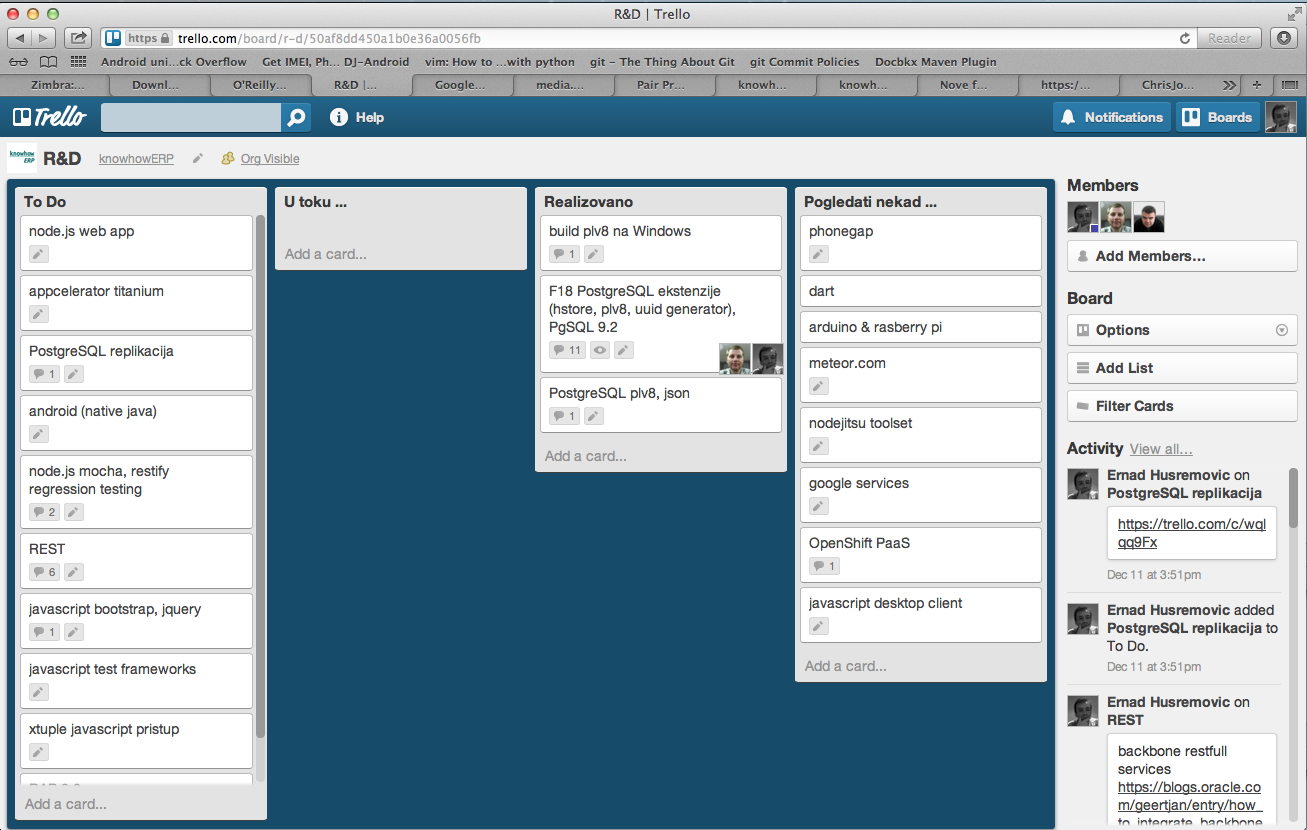
\includegraphics[width=14cm]{img/trello_rd.png}
\caption{Projekat: Research \& development}
\end{figure}

\begin{figure}[H]
\centering
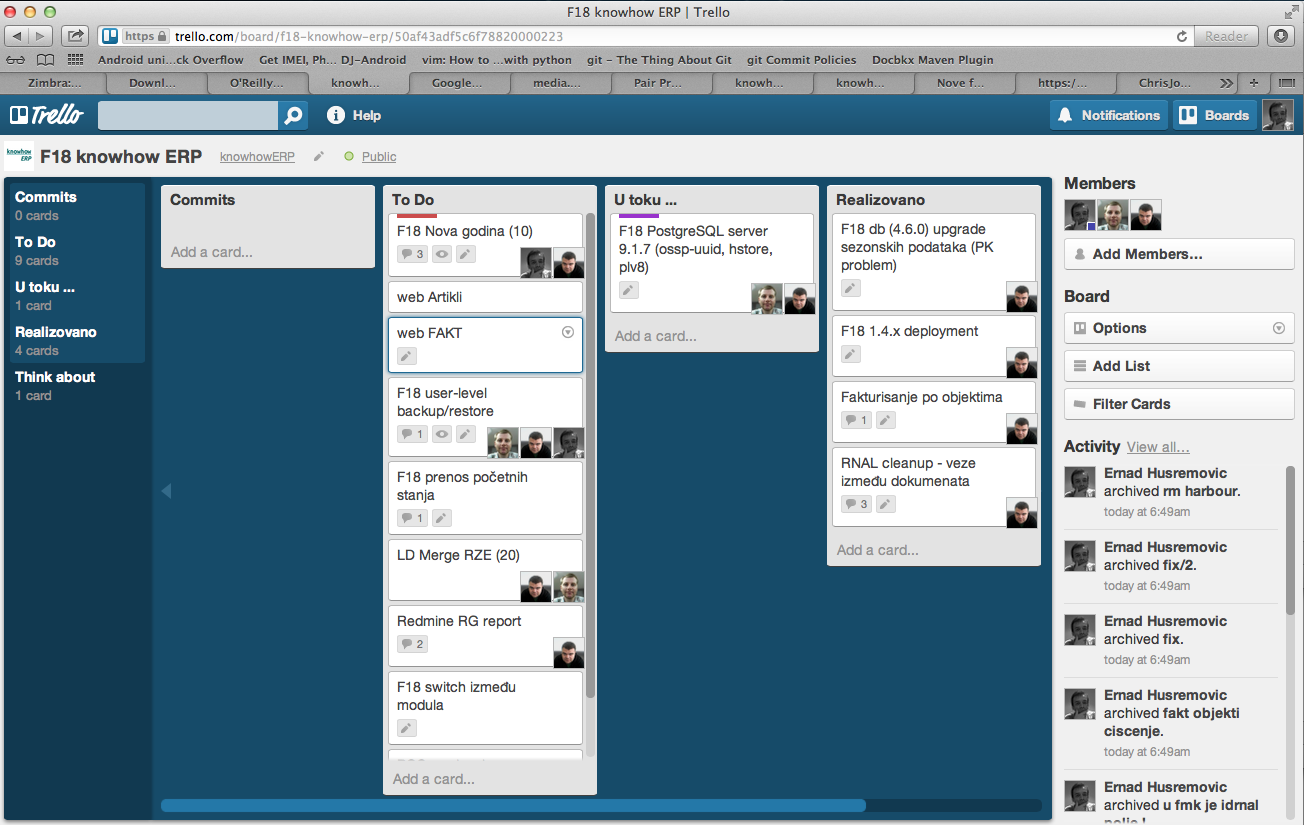
\includegraphics[width=14cm]{img/trello_f18.png}
\caption{Projekat: F18}
\end{figure}

\begin{figure}[H]
\centering
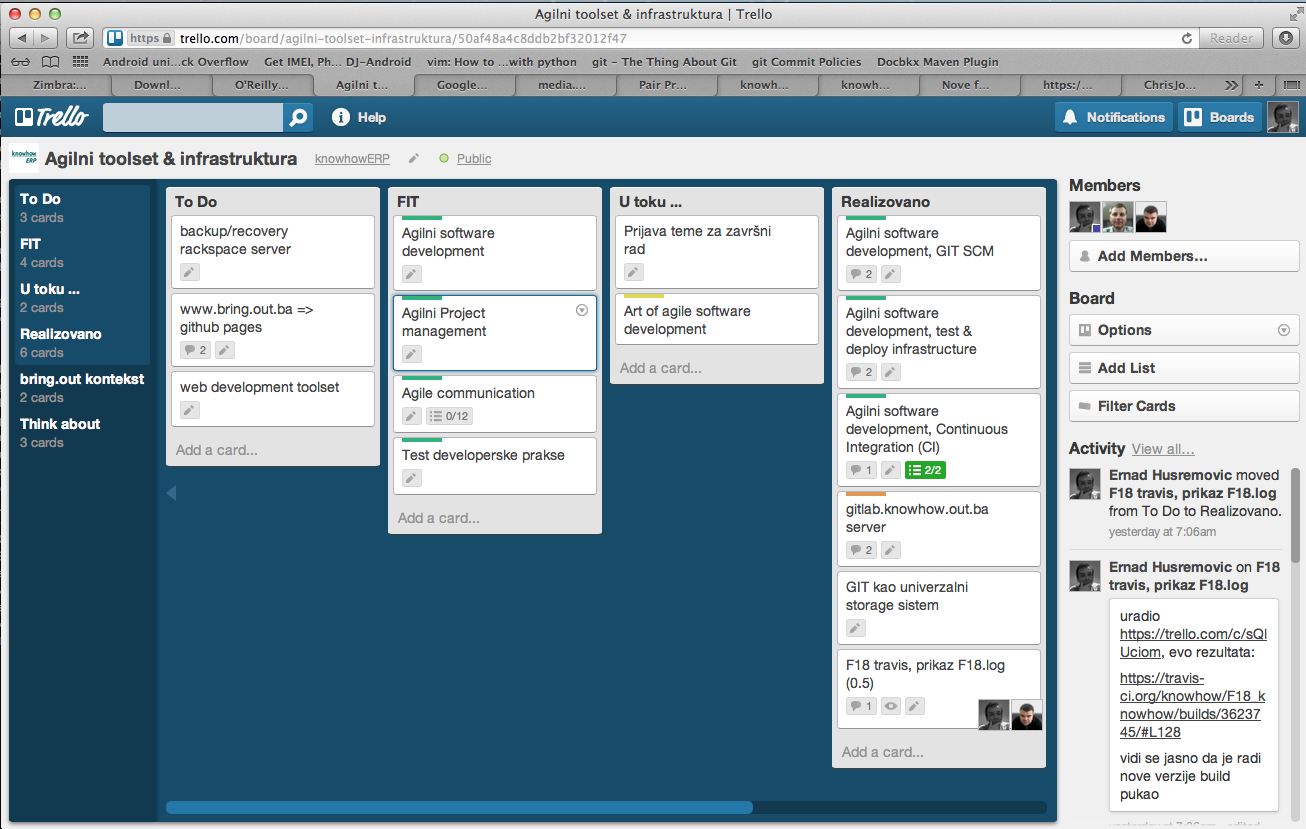
\includegraphics[width=14cm]{img/trello_agile.png}
\caption{Projekat: Agilni toolset}
\end{figure}

\begin{figure}[H]
\centering
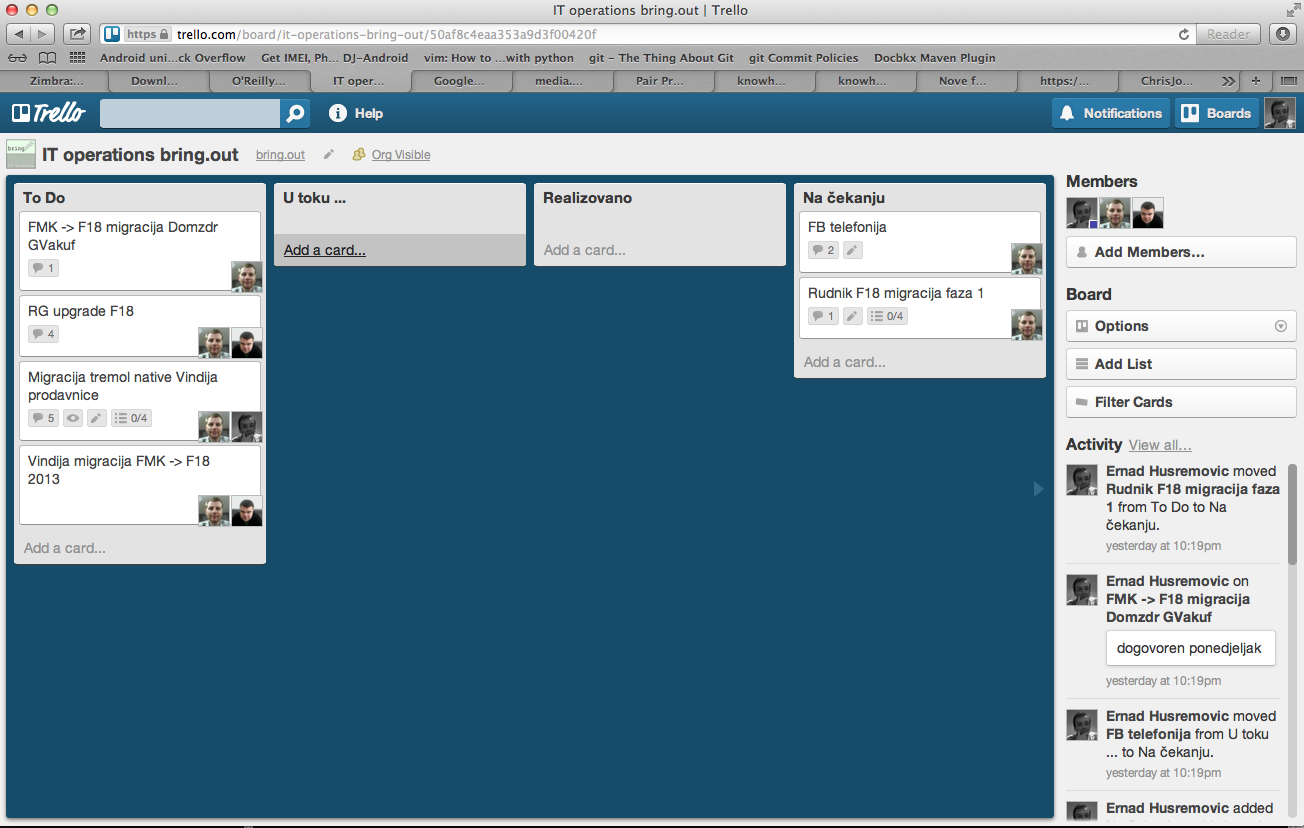
\includegraphics[width=14cm]{img/trello_ops.png}
\caption{Projekat: IT operacije bring.out}
\end{figure}

\section{Redmine project management}

\url{http://redmine.bring.out.ba/projects/f18} 

\chapter{Dizajn}

\section{Papir, olovka, bojice}

Skiciraj kako god ti odgovara. Bitno je da zadovolji svrhu - da prezentuje ideju, rješenje, koncept.

\begin{figure}[H]
\centering
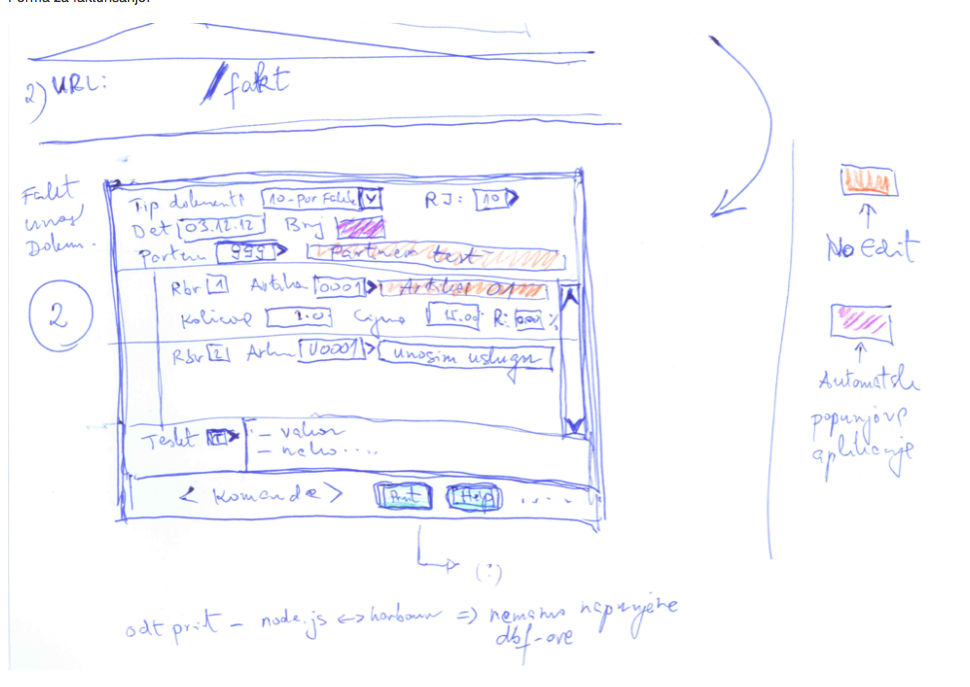
\includegraphics[width=14cm]{img/papir_i_olovka.png}
\caption{Papir, bojice, olovka}
\end{figure}

Primjer korištenja: \href{https://github.com/knowhow/F18_knowhow/wiki/F18-web-fakt}{\color{blue}{web FAKT UI prototip}}

\section{PlantUML}

\begin{figure}[H]
\centering
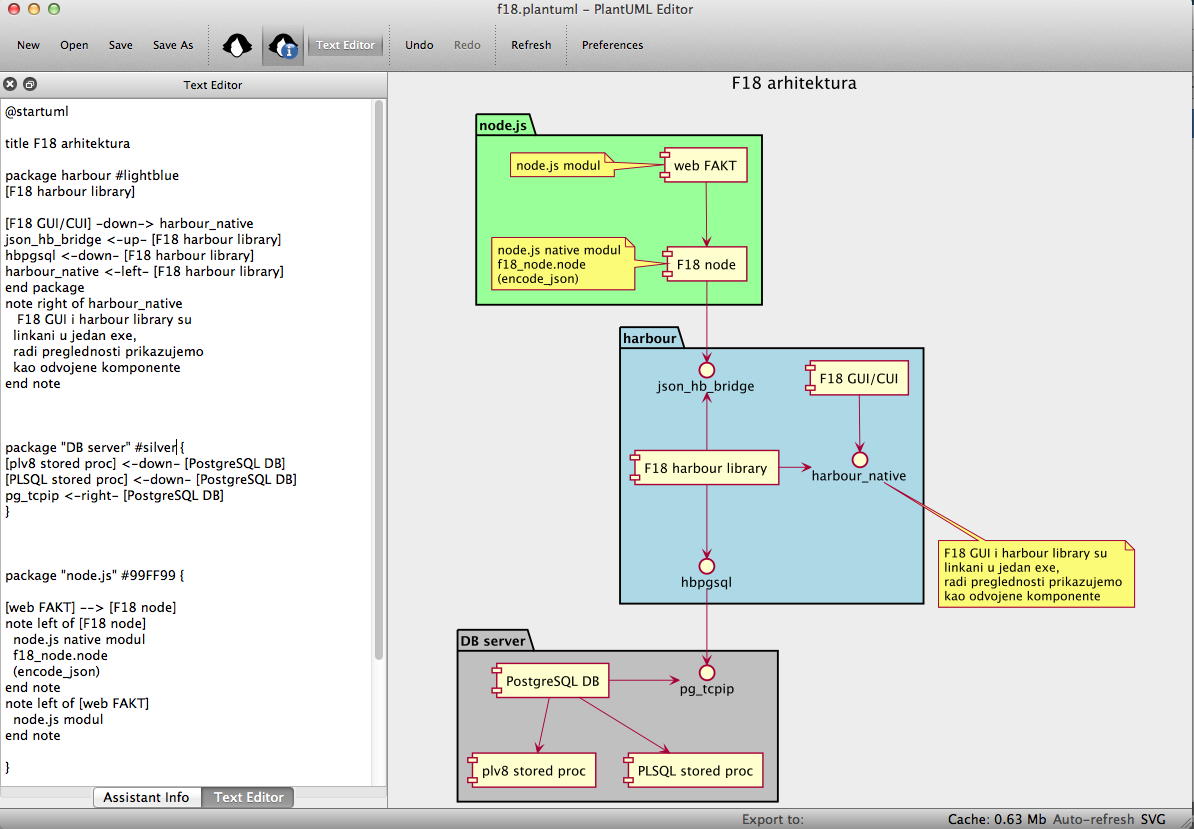
\includegraphics[width=14cm]{img/plantuml_f18.png}
\caption{Plant UML}
\end{figure}

Primjer korištenja: \href{https://github.com/knowhow/F18_knowhow/wiki/F18-arhitektura}{\color{blue}{F18 arhitektura}}

Plantuml editor i plantuml.jar \href{http://code.google.com/p/knowhow-erp/downloads/list?can=2&q=plantuml}{\color{blue}{download}}

\section{Erwiz ER-dijagrami}

\begin{lstlisting}
# Using Erwiz 0.9.0
{title: "Syn2Stock ERD V3"; title-size: 20}

# Entities

[Item] {color:red}
 *Item ID
  Type
  SimpleItem
  ...  
  Sources
  Source ID*
  Location ID*
  Lending ID*

[Source]
 *Source ID
  Price
  ...
  Manufacturer

[Location]
 *Location ID
  ...
  Room
  Locker

[Lending]
 *Lending ID
  Borrowed by
  ...
  Reminder ID*

[Reminder]
 *Reminder ID
  Start Date
  ...
  Message
  Item ID*
  Lending ID*

[Event]
  *Event ID
  Event Type
  Date
  User
  Item ID*

[Attachment]
 *Attachment ID
  File
  External URL
  Private

[Electronic Part] {color:orange}
 *Electronic Part ID
  Value
  Item ID*

[Book] {color:orange}
 *Book ID
  Subtitle
  ...
  Summary
  About the Author
  Item ID*

# Relationships
[Item] *--* [Source]
[Item] 1--1 [Location]
[Item] 1--* [Lending]
[Item] *--* [Attachment]
[Reminder] ---- [Item]
[Event] *--1 [Item] <contains->
[Electronic Part] ---- [Item] <is a->
[Book] ---- [Item] <is a->
\end{lstlisting}

generacija dijagrama:

\begin{lstlisting}
erwiz$ bin/erwiz examples/example.txt erwiz_example.png
\end{lstlisting}

\begin{figure}[H]
\centering
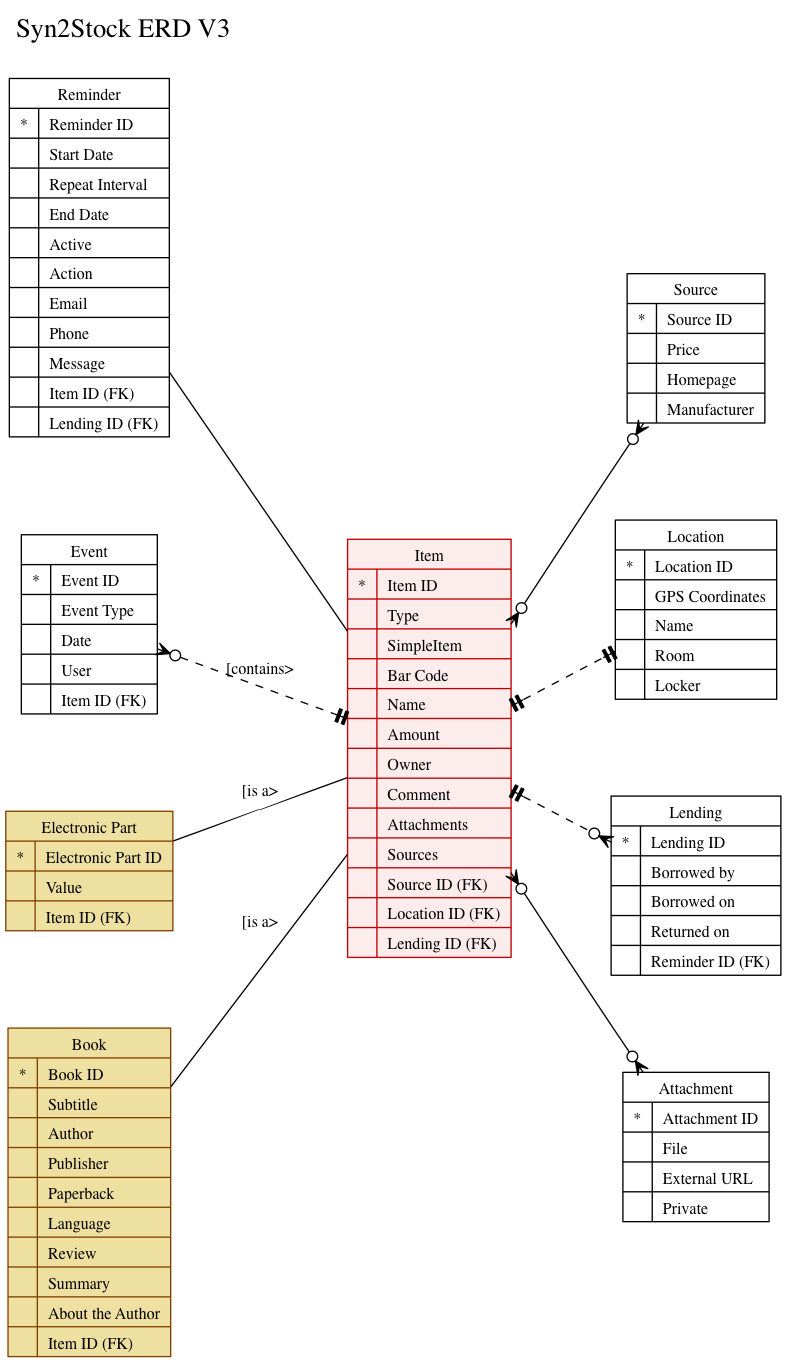
\includegraphics[width=12cm]{img/erwiz_example.png}
\caption{Erwiz E-R dijagram}
\end{figure}

Erwiz \href{http://code.google.com/p/knowhow-erp/downloads/list?can=2&q=erwiz}{\color{blue}{download}}

\chapter{Pisanje izvornog k\^oda, dokumentacija}

\section{Tekst editor}

\subsection{vim - konzolni tekst editor}

\begin{figure}[H]
\centering
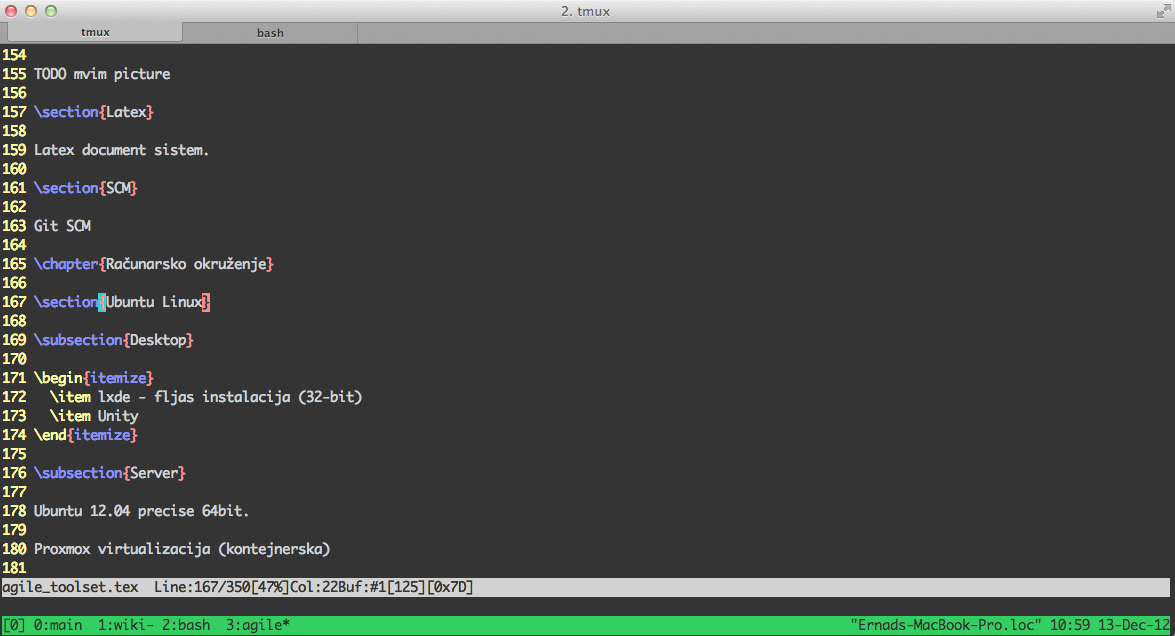
\includegraphics[width=14cm]{img/vim.png}
\caption{vim}
\end{figure}

\subsection{gvim/mvim - grafički tekst editor}

\begin{figure}[H]
\centering
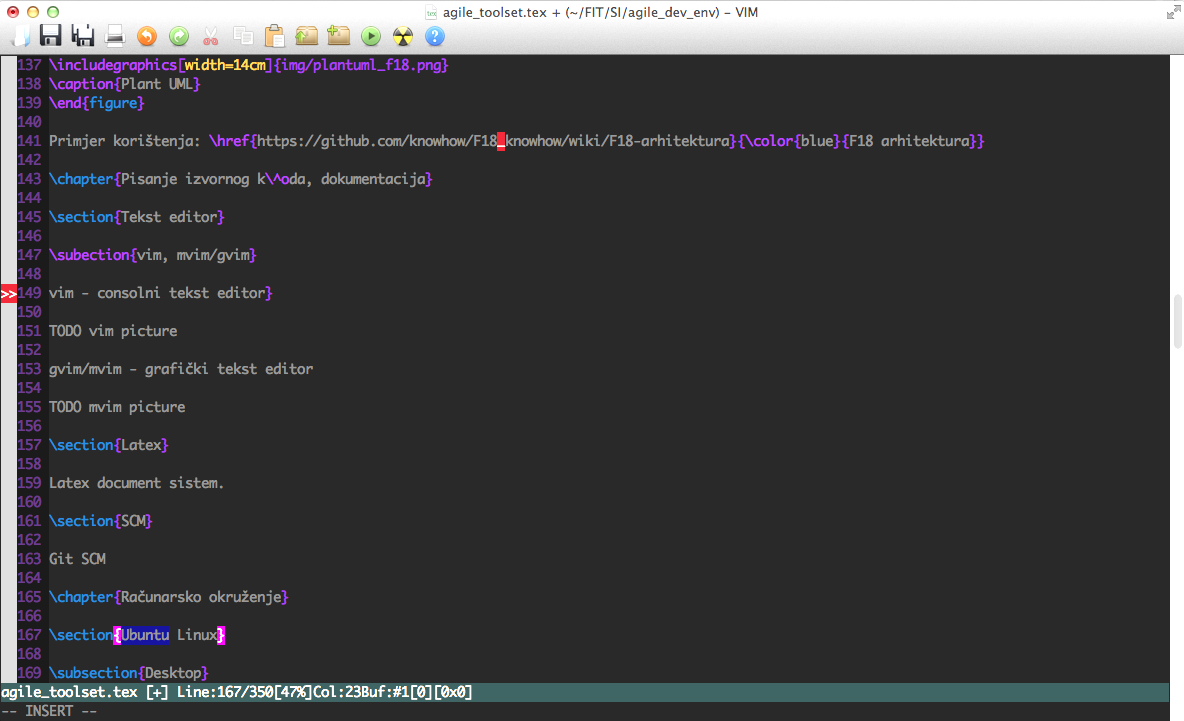
\includegraphics[width=14cm]{img/mvim.png}
\caption{mvim, Mac OS X grafička verzija vim editora}
\end{figure}

\subsection{notepad++}

Notepad++ za Windows OS.

\section{Latex}

Latex document sistem.

\section{SCM}

Git SCM

\section{Appcelerator Titanium IDE}

\begin{figure}[H]
\centering
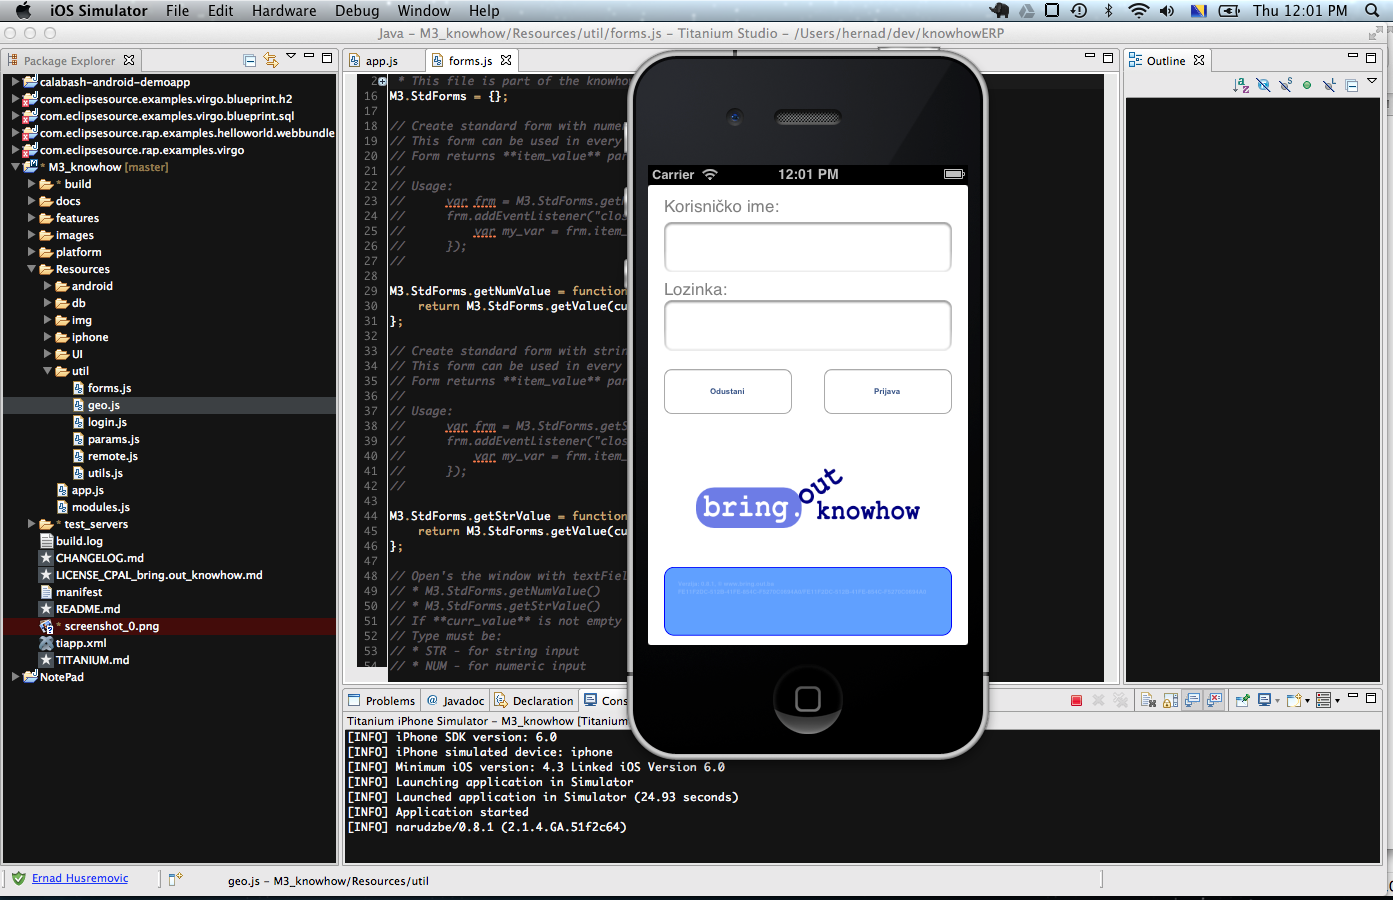
\includegraphics[width=14cm]{img/titanium_m3.png}
\caption{Appcelerator IDE, razvoj M3 mobilnog klijenta}
\end{figure}


\chapter{Računarsko okruženje}

\section{Ubuntu Linux}

\subsection{Desktop}

\begin{itemize}
  \item lxde - fljas instalacija (32-bit)
  \item Unity
\end{itemize}

\subsection{Server}

Ubuntu 12.04 precise 64bit.

Proxmox virtualizacija (kontejnerska)

\section{Mac OS X}

Developersko okruženje

\section{Windows OS}

Radi testiranja Windows OS verzija F18.

Uobičajeno se koristi unutar developerske virtualbox sesije.

\chapter{Testiranje}

\section{Oracle Virtualbox}

Vbox

\section{vagrant}

Vagrant vbox + test

\section{chef}

Chef configuration management

\chapter{Programski jezici}

\section{bash}

Administracijske i instalacijske skripte.

Stepen korištenja: \emph{4}

\section{SQL}

PostgreSQL dijalekt.

Nivo korištenja: 3

\section{javascript}

\subsection{browser}

Nivo korištenja: 0

\subsection{node.js}

Nivo korištenja: 0

\subsection{appcelerator titanium javascript}

Mobilni (hibridni) klijent

Nivo korištenja: 2

\subsection{android java}

appcelerator ekstenzije, sporadično se koristi.

Nivo korištenja: 1

\section{harbour}

F18 izvorni k\^od.

Nivo korištenja: 5

\section{HTML, CSS}

Nivo korištenja: 0

\section{C/C++}

Uglavno kao bridge jezik za različite tehnologije (harbour-node.js, ruby ekstenzije za alarm sistem)

Nivo korištenja: 3

\subsection{xTuple source}

knowhowERP GUI klijent (xTuple) je pisan (core sistem) u C/C++. Međutim, taj klijent se ne razvija aktivno.

Updater koji se koristi za migraciju F18 se svakodnevno koristi (ali se sam updater rijetko mijenja)

\section{java}

Postoje bitni ''java'' bazirani projekti koji se intenzivno koriste:
\begin{itemize}
 \item zimbra
 \item jod-reports
\end{itemize}

Međutim, sam programski jezik se ne koristi u razvoju.

Nivo korištenja: 0

\section{ruby}

Koristi se uglavnom za pomoćne operacije. 

Postoje stariji projekti rađeni u ruby-ju (alarm)

Nivo korištenja: 3

\section{python}

Malo se koristi. 

Postoje stariji projekti rađeni u python-u (sql\_synchro)

Nivo korištenja: 2

\chapter{Frameworks}

\section{Twitter bootstrap}

\section{express node.js}

\chapter{Test programer frameworks}

\section{node.js testing frameworkds}

\subsection{Jasmine}

Browser, node.js

\subsection{vows}

\subsection{mocha}

\url{http://visionmedia.github.com/mocha}


\chapter{Database alati}

\section{PostgreSQL}

\subsection{PgAdmin}

PostgresSQL GUI konzola

\subsection{psql}

postgresql konzolna aplikacija

\subsection{Postgres.app}

Mac OS X \url{http://postgresapp.com}

Ekstenzije:
\begin{itemize}
  \item hstore
  \item plv8
  \item ossd-uuid  
\end{itemize}

\chapter{Ostali alati}

\section{konzola}

\subsection{tmux - Terminal multiplekser }

\begin{figure}[H]
\centering
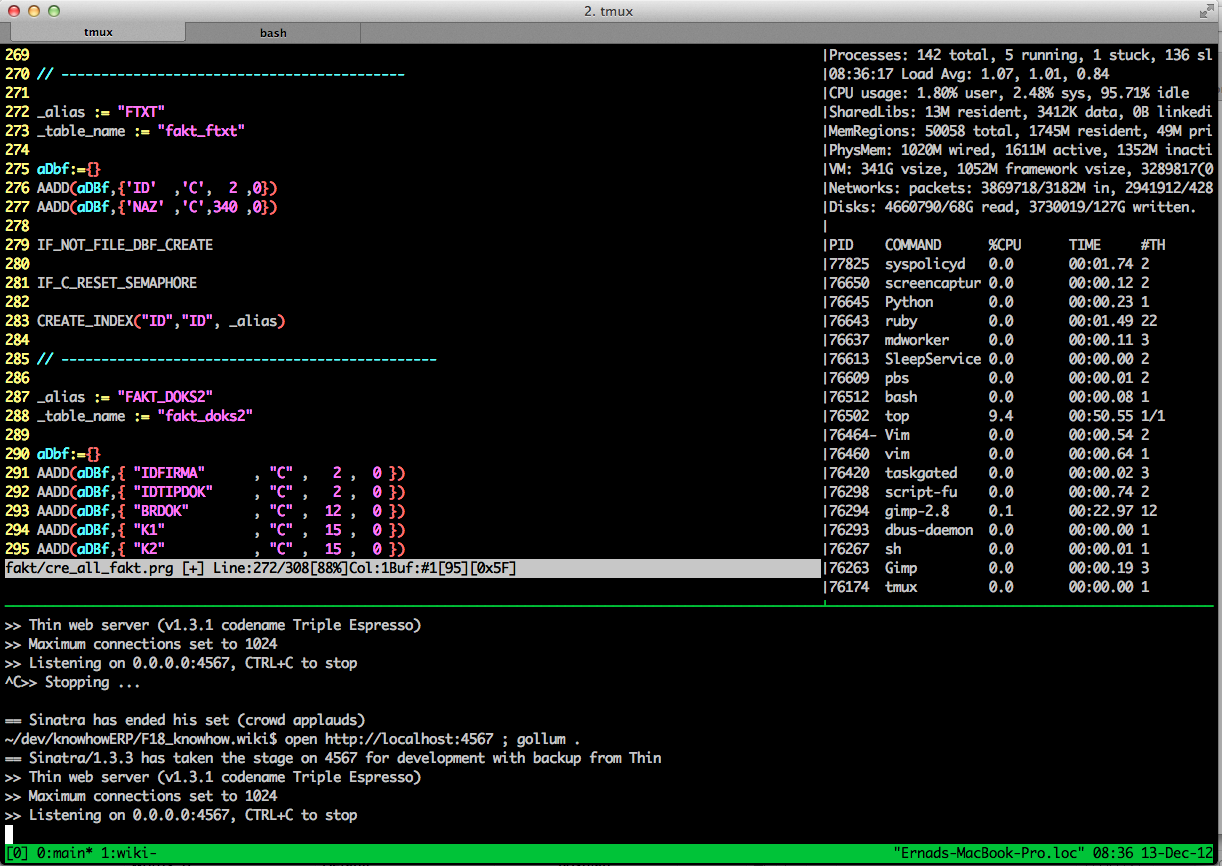
\includegraphics[width=14cm]{img/tmux.png}
\caption{tmux}
\end{figure}


\section{ssh, scp}

Remote pristup ubuntu linux serverima.

\section{rsync}

\section{Pretraga}

\subsection{Grep, ack, sed}

ack, grep

\subsection{vgrep}

Pretraga unutar vi editora

\chapter{Grafička obrada}

\section{Video editing}

QuickTime screen capture (Mac OS X)

\section{Bitmap picture}

Gimp

\section{Vector picture}

Inkscape

\chapter{Uredske aplikacije}

\section{LibreOffice}

Writer, Calc, rijetko Impress

\section{zimbra email}

\chapter{Internet provajderi}

\section{Google code, downloads servis}

\begin{itemize}
  \item \url{http://code.google.com/p/knowhow-erp/downloads/list}
  \item \url{http://code.google.com/p/knowhow-erp-f18/downloads/list}
  \item \url{http://code.google.com/p/knowhow-erp-fmk/downloads/list}
\end{itemize}

\section{Github, GIT repozitorij, WikiPages }

\begin{itemize}
  \item GIT repozitorij \url{https://github.com/knowhow/F18_knowhow}
  \item Github WikiPages \url{https://github.com/knowhow/F18_knowhow/wiki} 
\end{itemize}

\section{Travis CI}

\begin{itemize}
  \item \url{https://travis-ci.org/knowhow/F18_knowhow}
\end{itemize}

\section{Youtube video materijali}

Youtube bringoutba kanal koristimo \url{http://www.youtube.com/user/bringoutba}. Koristi se za prezentacije:
\begin{itemize}
 \item Unutar razvojnog tima
 \item Za krajnje korisnike
\end{itemize}

\section{Rackspace}

Cloud hosting provjader

\section{Blogiranje}

Posterous:

\begin{itemize}
  \item \url{http://www.bring.out.ba}
  \item \url{http://do-we-know-how.bring.out.ba}
\end{itemize}


\chapter{Korišteni formati podataka}

\section{txt}

Plain text format.

\subsection{Markdown markup jezik}

Github WikiPages, README projekata

\subsection{(La)tex}

Latex format

\section{OASIS open document format (ODT)}

odt, ods

\section{json}

Data exchange format.  Pogodan i za konfiguracijske datoteke.

\section{PDF}

PDF - de-facto standard za razmjenu dokumenata.

\section{PNG}

png grafički bitmap format

\section{SVG}

Inskape svg, standard internet SVG


% -------------------------------------------------
%\bibliography{literatura}
%\bibliographystyle{fit}

\end{document}
